%%%%%%%%%%%%%%%%%%%%%%%%%%%%%%%%%%%%%%%%%%%%%%%%%%%
% gamma.tex 
% Coordinator J. M. C. Brown
%%%%%%%%%%%%%%%%%%%%%%%%%%%%%%%%%%%%%%%%%%%%%%%%%%%
% \begin{figure}
% 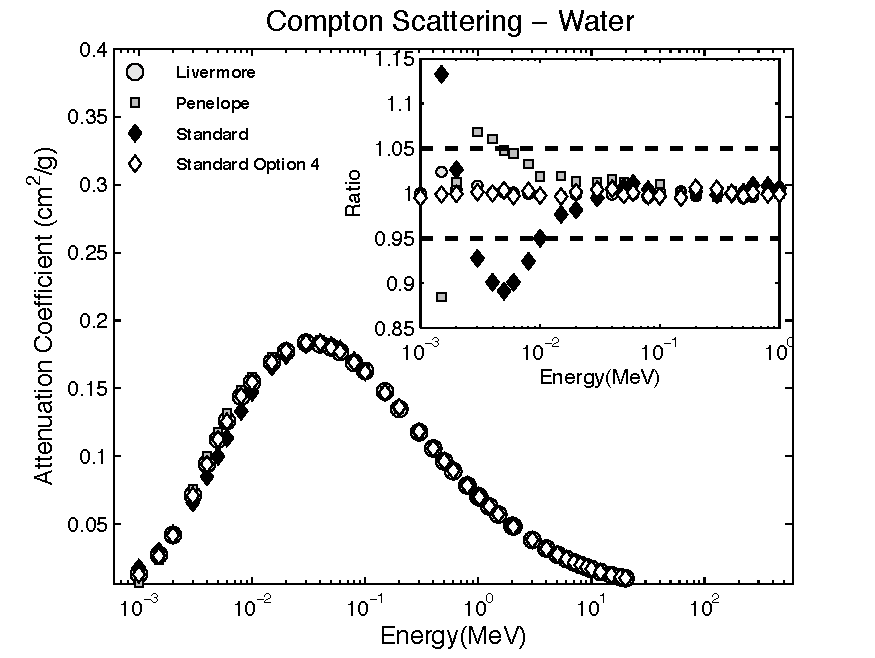
\includegraphics[width=0.5\textwidth]{figures/plot_compton.pdf}
% \caption{Compton scattering attenuation coefficient, calculated for different
%          \Gfour{} models. \gclass{G4LowEPComptonModel} is used in the Option4
%          EM physics configuration.  The inset shows the ratio of the coefficient
%          calculated using each alternative \Gfour{} electromagnetic physics list,
%          to the value from NIST XCOM \cite{embib:gamma16}.  The 
%          dashed lines correspond to a $\pm 5$\% difference.}
% \label{em:compton}
% \end{figure}
The basic set of gamma models in the EM physics packages includes models
developed for HEP applications \cite{bib:G4}, models based on the Livermore
evaluated data library \cite{embib:epdl} and a C++ implementation of the 
Penelope 2008 model \cite{embib:pen}.  Recent releases of \Gfour{} have included
revised versions of existing models, and the addition of new gamma physics 
processes and models. The low and high energy models were improved and display
similar accuracy in their shared domain of validity \cite{embib:uni2}. 
These modifications not only increased model accuracy but increased 
computational efficiency and enabled sharing of internal physics tables, 
where possible, in MT mode \cite{embib:chep14}.  
New gamma models were added to take into account physics effects not available
previously in \Gfour{} or in other simulation codes. 

A new relativistic pair production model, 
\gclass{G4Pair\allowbreak{}Production\allowbreak{}RelModel}, was developed for
simulations in astrophysics, 
LHC experiments, and other HEP applications.  This model takes into account 
the Landau-Pomeranchuk-Migdal (LPM) effect \cite{embib:gamma5}, which describes
the decrease of pair production cross sections at ultra-relativistic energies 
for dense media \cite{embib:gamma6}.  This model is physically accurate only
above 100 MeV, as no lower energy corrections are included.  It is suggested for
use in HEP applications above 80 GeV.  The use of the relativistic model is 
essential for the accurate simulation of new physics at LHC.

Two new gamma conversion models were developed to take into account the effect
of gamma ray polarization:
\begin{itemize}
\item \gclass{G4LivermorePolarized\allowbreak{}GammaConversionModel} and
\item \gclass{G4BoldyshevTripletModel} (to be used in unison with
      \gclass{G4Livermore\allowbreak{}NuclearGamma\allowbreak{}ConversionModel}).
\end{itemize}
The first is responsible for sampling electron-positron pair production by 
linearly polarized gamma rays with energies above 50 MeV \cite{embib:gamma11},
while the second (currently valid only above 100 MeV) simulates the pair 
production process in the electron field with the emission of an 
additional recoil electron \cite{embib:gamma12}, properly taking into account 
the so-called ``triplet'' production total cross section.

The Livermore polarized gamma conversion model is based on the Heitler cross
section, where the azimuthal distribution of the pair was obtained by 
integrating the cross section over energy and polar angles \cite{embib:gamma11}.

The Boldyshev triplet model uses Borselino diagrams to calculate the cross 
sections \cite{embib:pol3}.  Most of the recoil electrons in the Boldyshev model
have low energy, with a peak around $8/(T/mc^2)$, expressed in MeV, where $T$
is the gamma energy and $m$ is the electron rest mass.  Thus, a model for the
cross section was developed including a momentum threshold value of 1 $mc$, in
order to avoid the generation of too many very low energy recoil electrons
\cite{embib:pol4}. 

Finally, a specialized Compton scattering model 
\gclass{G4Low\allowbreak{}EPCompton\allowbreak{}Model} was 
developed \cite{embib:gamma13,embib:gamma14}.  Through the implementation of a
theoretical foundation that ensured the conservation of energy and momentum in
the relativistic impulse approximation \cite{embib:gamma15}, this model
implements energy and directional algorithms for both the scattered photon and 
ejected Compton electron developed from first principles. It was developed to 
address the limited accuracy of the Compton electron ejection algorithms present
in other low energy Compton scattering models that have been observed below
5~MeV \cite{embib:gamma14,embib:gamma7,embib:gamma8}. Figure \ref{em:compton} 
shows the comparison of different \Gfour{} Compton scattering cross sections
versus NIST evaluated data \cite{embib:gamma16} calculated with the methodology 
described in \cite{embib:gamma17}.  The \gclass{G4LowEPComptonModel} agrees with
the reference data to within
1\%, the statistical uncertainty of the simulation results.  The Penelope and 
Standard models result in differences up to 10\% with respect to the NIST data
for energies between 2 and 10~keV.  At higher energies, the differences are 
smaller and are below 1\% above 100 keV, corresponding to the statistical 
uncertainty of the simulation results.
\begin{figure}
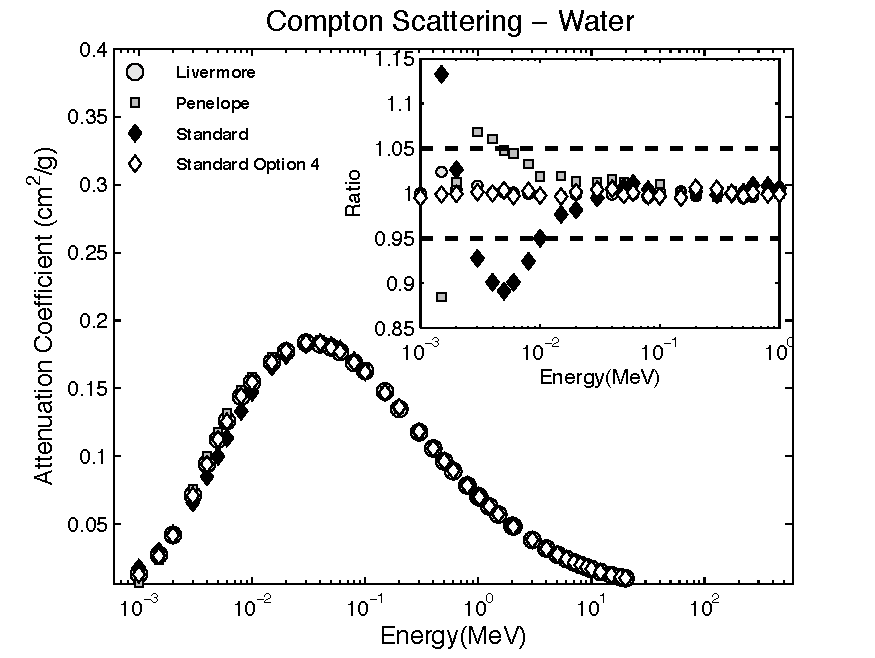
\includegraphics[width=0.5\textwidth]{figures/plot_compton.pdf}
\caption{Compton scattering attenuation coefficient, calculated for different
         \Gfour{} models. \gclass{G4LowEPComptonModel} is used in the Option4
         EM physics configuration.  The inset shows the ratio of the coefficient
         calculated using each alternative \Gfour{} electromagnetic physics list,
         to the value from NIST XCOM \cite{embib:gamma16}.  The
         dashed lines correspond to a $\pm 5$\% difference.}
\label{em:compton}
\end{figure}

